\chapter{Technik}
\label{technik}

Beim Tischfussball ist das Toreschiessen das wichtigste um zu Gewinnen und daher ist das Spiel von Anfängern durch viele schnelle (Direkt-)Schüße geprägt.
Vor allem durch Trichschüsse heben sich erfolgreichere Spieler hervor.
Im Amateur-Bereich kommen meist Pass- und Schuss-Optionen hinzu.
Und im Profi-Bereich werden meist alle Techniken angewandt, vor allem um strategisch eine Partie zu gewinnen. siehe nächstes Kapitel~\ref{taktik}. 
Bei allen Spielniveaus werden verschiedene Defensivtechniken angewandt, um die Offensive des Gegners erfolgreich zu verteidigen.
All diese Techniken sind notwendig für ein kontrolliertes Spiel -- was der eigentlich Trick der Profis ist.

Technik ist die Grundlage eines jeden Sports. 
Das Ziel einer sauberen Technik ist das Kontrollieren des Balles mit den Spielfiguren in unterschiedlichen Spielsituationen:
\begin{itemize}
    \item in der Offensive (Kapitel \ref{technik:offensive}) und bei Ballbesitz gibt es Techniken für 
        \begin{itemize}
            \item das Passen, 
            \item das Annehmen und 
            \item das Schießen des Balles
        \end{itemize}
    \item in der Defensive (Kapitel \ref{technik:defensive}) und bei Nicht-Ballbesitz gibt es Techniken für 
        \begin{itemize}
            \item das Stellungsspiel, 
            \item das Blocken und 
            \item das Fangen des Balles  
        \end{itemize}
\end{itemize}
Zunächst in Kapitel \ref{technik:haltung} wird die grundlegende Körper- und Griffhaltung beschrieben, wobei sich vor allem die Griffhaltung und Arm- und Oberkörperbewegung beim Spielen der Techniken verändern kann. 

\paragraph{Technik-Training;} 
Das Erlernen der Techniken und entprechendes Training sollte dem Spielniveau und dem Alter angepasst werden. 
Spielerisches Erlenen (siehe Kapitel~\ref{chap:spielformen}) ist etwa für Kinder und Jugendliche und Anfänger geeignet, regelmäßige Wettkämofe (Liga und Turniere) für Fortgeschrittene und statisches Techniktraining für ambitionierte Spieler.


%%%%%%%%%%%%%%%%%%%%%%%%%%%%%%%%%%%%%%%%%%%%%
\section{Körper- und Handhaltung}
\label{technik:haltung}

Bei Ballsportarten sind die Körperstellung und der Stand zum Ball eine Grundvorraussetzung zum erfolgreichen Spiel.
Bei Schlägersportarten sind die Handhaltung und die Arm- und Körperbeweglichkeit eine Grundvorraussetzung zur erfolgreichen Ausführung einer Spielaktion.
Diesen beiden Aspekte sind auch beim Tischfussball zu beachten:
Ein richtiger Stand zum Tisch beinhaltet eine eine lockere Grundbeweglichkeit von Körper und vor allem den Armen und Händen zum Bewegen der Stangen (Kapitel~\ref{technik:haltung:koerper}),
Eine richtige Handhaltung der Stangen umfasst das einer Spielsituation bedingtes Drehen und Schieben und Ziehen der Stangen und damit Spielen des Balles (Kapitel~\ref{technik:haltung:griffe}).
Die folgenden Kapitel geben eine grundlegende Richtlinie zur richtigen Haltung, die für jeden individuell anders ist. 

\begin{figure}
    \centering 
        \begin{subfigure}[b]{0.9\textwidth} 
            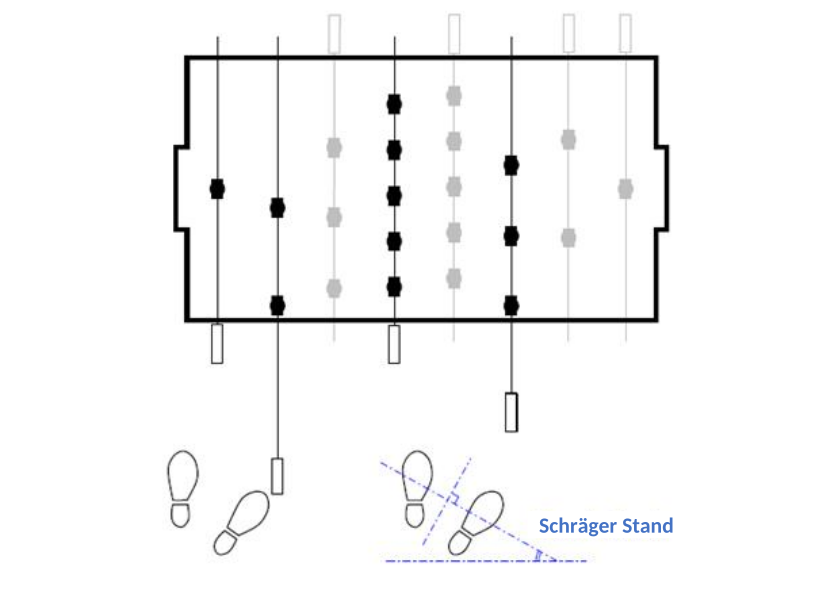
\includegraphics[width=\textwidth]{img/haltung_koerper.png} 
            \caption{Grundlegender Körperstand} 
            \label{fig:haltung:koerper} 
            \vspace{0.5cm}
        \end{subfigure} 
        \begin{subfigure}[b]{0.5\textwidth} 
            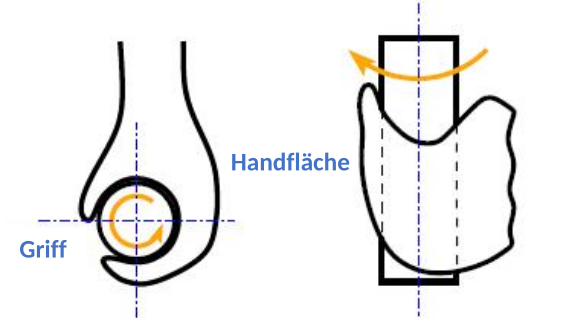
\includegraphics[width=\textwidth]{img/haltung_hand.png} 
            \caption{Grundlegende Handhaltung} 
            \label{fig:haltung:hand} 
        \end{subfigure} 
        \label{fig:haltung} 
        \caption{Die grundlegenden Haltungen [\cite{itsf_basics}]} 
\end{figure}

%%%%%%%%%%%%%%%%%%%%%%%%%%%%%%%%%%%%%%%%%%%%%
\subsection{Körperhaltung}
\label{technik:haltung:koerper}

Die Grundhaltung ist ein schulterbreiter Stand.
Der Abstand vom Körper zum Tisch mit einem leichten schrägen Stand mit Blick zum Tor (siehe Abbildung \ref{fig:haltung:koerper}) sollte so sein, dass die Stangen beweglich ganz rein- und rausgefahren und gedreht werden können.
Dabei kann der rechte Arm aus der Schulter seitlich am Körper vor und zurück bewegt werden. 

Ein lockerer Stand sollte die Arme für flüssige Stangenbewegungen entlasten. 
Daher sollte man sich etwa nicht auf den Griffen abstützen.
Hierbei hilft es leicht in die Knie zu gehen und das Körpergewicht leicht auf die Fussballen zu verlagern; der Oberkörper ist meist gebeugt zum Tisch, dabei sollte der Rücken einigermaßen gerade und die Schultern locker sein.

Diese Grundhaltung ist statisch, dass bedeutet die Füße behalten ihre Position. 
Meist wird diese statische Haltung weitestgehend bei der Ausführung eines Passes oder Schusses beibehalten. 
Leichte Positionsänderungen passieren für einen angepassten Stand etwa für eine bestimmte Schusstechnik (Zieher, Schieber, Abroller/Front-Pin) und Defensivtechniken.
Und in der Einzeldisziplin muss der Spieler sich am Tisch ständig bewegen und seine Position der jeweiligen Ballposition bzw. der gewollten Stangenkontrolle anpassen.

\paragraph{Hinweis:} Um Rückenproblemen vorzubeugen, sollte neben der entspannten Körperhaltung eine Ausgleichsbewegung vor oder nach dem Tischfussballspielen gemacht werden.
Das kann eine andere Sportart sein, aber auch schon ein paar kurze Aufwärm- und Lockerungsübungen können entspannen: Hüpfen, Armkreisen, Luftklettern, usw. 

%%%%%%%%%%%%%%%%%%%%%%%%%%%%%%%%%%%%%%%%%%%%%
\subsection{Handhaltung}
\label{technik:haltung:griffe}

Die standardmäßige Handhaltung ist eine geschlossene
und der Handrücken zeigt dabei nach oben (siehe Abbildung~\ref{fig:haltung:hand}).
Wird der Griff so gehalten, wenn gleichzeitig die Figuren mit den Füßen nach unten stehen, kann die Stange durch Bewegen des Handgelenks so gedreht werden, dass die Füße der Figuren die volle Drehbereich Abfahren (siehe Abbildung~\ref{fig:figurdrehen}):
\begin{itemize}
    \item von ganz hinten, um einen \textit{Ball hinter der Stange} zu spielen (Hinten Klemmen, Back-Pin, Brush/Drücker, Druckpunkt, Fangen, siehe Kapitel \ref{}), über
    \item gerade Figuren-Position für Tic-Tac (Kapitel \ref{}) die volle Abdeckung (Kapitel \ref{}) bis 
    \item ganz vorne, um einen \textit{Ball vor der Stange} zu spielen (Vorne Klemmen, Front-Pin, Fangen, siehe Kapitel \ref{}).
\end{itemize}

\begin{figure}
    \centering 
        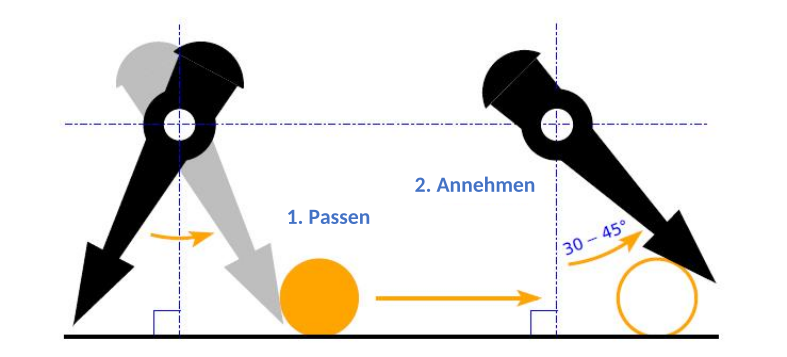
\includegraphics[width=0.7\textwidth]{img/haltung_figur.png} 
        \caption{Drehung der Stange: Verschiedene Figurpositionen, hinter der Stange (links), rechts vor der Stange (rechts) [\cite{itsf_basics}]} 
        \label{fig:haltung:figur} 
\end{figure}

Der Griff wird je nach Technik unterschiedlich stark festgehalten oder mit verschiedenen Drehgeschwindigkeiten bewegt. 
Grundsätzlich lässt  eine lockere Handhaltung die Stange in den Lagern frei und damit letztendlich schnell bewegen.
Das gilt für Seitwärts-Bewegungen der Stange und für Drehbewegungen der Stange.

Je nach Körperhaltung und Position, ist der Unterarm unterschiedlich geneigt und damit die Achse des Handgelenks unterschiedlich zur Drehachse der Stange.
Hier gibt es Anpassungen je nach Technik (Zieher, Schieber, Linke-Hand-Pass, Defensiv-Stellungen) oder nach indivueller Haltung.

Eine erste abweichende Griffhaltung ist der Fingergriff: Hierbei halten die Fingerspitzen das Griff Ende, der Unterarm ist fast waagrecht, und die Stange kann aus dem Unterarm schnell gedreht werden.
Für die Schusstechniken Abroller/Front-Pin und Jet gibt es eine komplett andere Grundhaltung des Griffs, siehe Kapitel~\ref{} bzw. \ref{}.


%%%%%%%%%%%%%%%%%%%%%%%%%%%%%%%%%%%%%%%%%%%%%
%%%%%%%%%%%%%%%%%%%%%%%%%%%%%%%%%%%%%%%%%%%%%
\section{Offensive: Passen, Annehmen, Schiessen}
\label{technik:offensive}

Beim Tischfussball ist die \gls{offensive} bei Ballbesitz möglich.
Dabei können die Figuren durch Bewegen der Stange nur im jeweiligen Bereich den Ball erreichen und spielen (vergleiche Abbildung~\ref{fig:tischbereiche}).
Ballkontrolle oder Ballgefühl beinhalten das Passen, das Annehmen und das Schiessen des Balles.



%%%%%%%%%%%%%%%%%%%%%%%%%%%%%%%%%%%%%%%%%%%%%
\subsection{Ballführung (auf einer Stange)} 
\label{technik:offensive:eine}

Figur zum Ball: Spielen und annehmen

\begin{itemize}
\item Ruhender Ball und Puppenwechsel.
\item Tictac oder Vorne-hinten Klemmen.
\item Auf der 2er-Stange zwischen der 1. und der 2. Puppe.
\item Auf der 3er-Stange zwischen der 1. und der 2. Puppe oder der 2. und der 3.Puppe oder mit der 1. und 3. Puppe.
\item Auf der 5er-Stange zwischen der zwei benachbarten Puppen oder mit zwei Puppen und dabei eine Puppe auslassen.
\end{itemize}


%%%%%%%%%%%%%%%%%%%%%%%%%%%%%%%%%%%%%%%%%%%%%
\subsection{Passen (zwischen zwei Stangen)}
\label{technik:offensive:zwei}

Figur zum Ball: Spielen und annehmen

\begin{itemize}
\item Spielprinzipien: Ins Feld, gerade oder an die Bande.
\item Passtechniken: Kanten-, Stick und Brushpass. 
\href{http://ungeblogtkickern.blogspot.de/2015/09/schrag-schieen.html}{Artikel auf Ungeblogt}
\item Annahmetechniken: Ballanahme.
\end{itemize}

Passmöglichkeiten:
\begin{itemize}
\item Von der 5er- auf die 3er-Stange.
\item Von der 2er-Stange auf die 3er-Stange.
\item Von der 2er-Stange auf die 5er-Stange.
\end{itemize}


%%%%%%%%%%%%%%%%%%%%%%%%%%%%%%%%%%%%%%%%%%%%%
\subsection{Torschüsse}
\label{technik:offensive:torschuesse}

\begin{itemize}
\item Schussprinzipien: Schneller als der Gegner, Seitwärtsbewegung und Schussbewegung. Für Fortgeschrittene: Geschwindigkeit, Präzision, Konstanz, Abrufbarkeit
\item Schusstechniken: Schieber/Zieher, \href{http://ungeblogtkickern.blogspot.de/2014/07/schritt-fur-schritt-pin-schieen.html}{Abroller/Pin} oder Jet.
\item Von der 3er-Stange oder der 2er-Reihe.
\item Trickschüsse
\end{itemize}





%%%%%%%%%%%%%%%%%%%%%%%%%%%%%%%%%%%%%%%%%%%%%
%%%%%%%%%%%%%%%%%%%%%%%%%%%%%%%%%%%%%%%%%%%%%
\section{Defensive: Stellen, Blocken, Fangen}
\label{technik:defensive}

\begin{itemize}
\item Defensiv-Prinzip: mit den Figuren die direkten Ballwege zum Tor blockieren (Seitwärtsbewegung)  
\item Klapprichtung der Figuren und Abstand der Figuren (Drehbewegung)
\item Bälle blocken, fangen, annehmen 
\end{itemize}
Daraus folgen grundlegende sogenannte Stellungsspiele.


\subsection{Ballbesitz des Gegners im Abwehrbereich}
\label{technik:defensive:gegnerabwehr}

\begin{itemize}
\item Deckung als Stürmer
\item Deckung als Torwart: (statisch) im kurzen/langen Eck
\item Deckung im Doppel
\item Deckung im Einzel
\end{itemize}


\subsection{Ballbesitz des Gegners im Mittelfeld (5er-Reihe)}
\label{technik:defensive:gegnermittelfeld}

\begin{itemize}
\item Deckung als Stürmer (5er-Reihe): Pass verhindern, kleinster Fahrbereich, an die Bande fahren
\item Deckung als Torwart: Torschüße, direkter Ballweg
\end{itemize}


\subsection{Ballbesitz des Gegners im Sturm (3er-Reihe)}
\label{technik:defensive:gegnersturm}

\begin{itemize}
\item Deckung als Torwart: Reaktion, fahren, shaken, Wechseln
\end{itemize}

